%!TEX root = karulf-thesis.tex
\chapter{Human-Computer Interaction} % (fold)
\label{chapter:hci}
Human-Computer Interaction (HCI) is the study of how humans interface with technology. This includes traditional interfaces, such as graphical user interfaces controlled with a mouse and keyboard, as well as alternative interfaces such as the accelerometers in the Nintendo Wii™ controller or the motion tracking system in the Microsoft Kinect™.

Despite the advances in efficacy and popularity of non-traditional devices, this paper will be limited to standard devices found on most computer systems, e.g., a monitor, mouse, and keyboard. In Section~\ref{section:futurework} we will briefly highlight how alternative interfaces would enhance our proposed interface.

\section{Video Game Interfaces} % (fold)
\label{sec:video_game_interfaces}
Originally created as an application of computer graphics for use in the entertainment industry, video game development has matured into an independent industry in its own right. The popularity of video games has grown significantly throughout the past decade. The Entertainment Software Association estimates 68\% of American households now play computer or video games \cite{ESA}. This large demographic represents a pool of users already versed in exploring 3D virtual worlds interactively. In these interactions, users are not only perceiving the virtual world through simulated senses, but users are also performing actions and controlling their presence in the virtual world through input devices, eg., a mouse and keyboard.

\subsection{Video Games in Research} % (fold)
\label{sub:video_games_in_research}
Due to their common ancestry with human-computer interaction, many of the principles of video game design can be applied to the field of human-robot interaction (HRI), which will be discussed further in Section~\ref{sec:hri}. There are several published applications of video games within the fields of artificial intelligence and machine learning. We will explore two applications that leverage human resources to complement artificial intelligence.

Von Ahn concluded that video games can be an effective tool for generating training data sets for machine learning \cite{GWAP}. Von Ahn developed special video games he labeled ``games with a purpose.''  Such games provide a means to solve problems often considered trivial for humans, yet simultaneously considered quite challenging for computers. The \emph{ESP Game}, Von Ahn's first game, uses human computation to classify images that computer algorithms are unable to recognize. In these games, the interaction of the human and the computer has changed to include the human in the computation of data. This is an interesting inversion of traditional autonomy, where the human is given tasks by the computer's artificial intelligence \cite{GWAP}.

Grollman, in his dissertation work, applied a video game interface with HRI principles to capture training data for robotic user interfaces \cite{Grollman}. His application, RGame, recorded user’s actions as they controlled a robotic dog and taught it to play soccer. Grollman created an AI model for shooting and defending tasks, which utilized the aggregate of data collected from RGame. Similar to Von Ahn's research, the RGame interface allowed the computer request information from the user to help it solve a problem \cite{Grollman}.
% subsection video_games_in_research (end)

\subsection{First-Person \& Third-Person Games} % (fold)
\label{sub:first_person_games}
First-person games involve the direct control of a single character by the player. The game world is rendered from the viewpoint of that character, often with additional game information overlaid upon it. 

The majority of the interface is occupied with a rendering of the world from the character’s perspective. The player can only see what the character can see, and the viewpoint is fixed. Additional game information is overlaid in the manner of a heads-up display.

The challenge of first-person games is to build a situational awareness of the unseen elements of the surrounding environment. While this limited perspective often leads to exciting and engaging gameplay, it is a design choice that explicitly limits situational awareness.

Third-person games are similar, except the viewpoint is typically located above and behind the character. The viewport in third-person games follows the character as she moves through the world. Third-person games allow the player to see the character in the world and yields a greater sense of context. However, the viewpoint is still fixed, forcing the player to reconstruct unseen parts of the world in the player's mind.

Figure~\ref{fig:halo3} shows the user interface for \emph{Halo 3}, a recent first-person game \cite{Halo3}. The bottom left shows a local map, with the locations of other players and adversaries, while character and weapon status is displayed along the top. 

\begin{figure}[ht]
\begin{center}
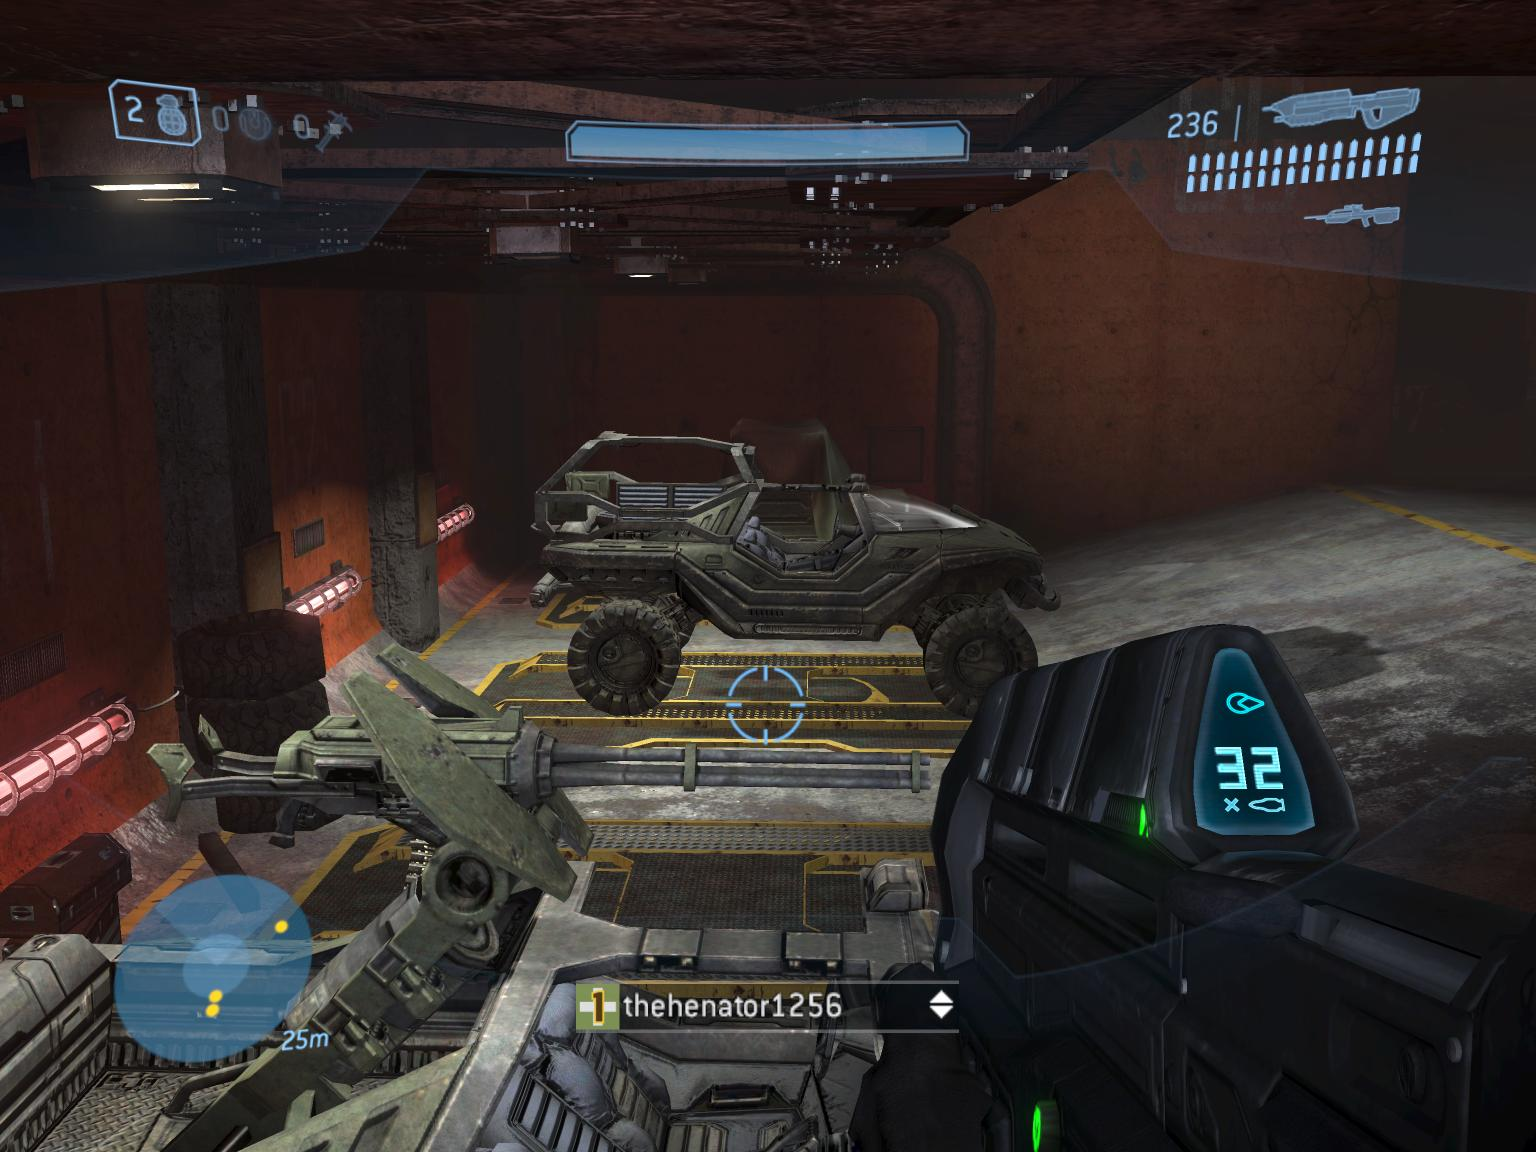
\includegraphics[width=5in]{images/halo3.jpg}
\caption{Bungie's \emph{Halo 3}: A first-person interface \label{fig:halo3}}
\end{center}
\end{figure}


\subsection{Real-Time Strategy Games} % (fold)
\label{sub:RTS_games}

% RTS games are full genre in the world of computer and video games. The goal of real-time strategy games is to effectively control your units to achieve a specified goal. Often these goals require the user to control units across a large  map. Real-time strategy games stress a users ability coordinate large numbers of units in a short amount of time. 

% RTS games use an isomorphic top-down view to display a large section of the environment at a time. The map can be navigated using either the keyboard or the mouse. Placing the moue pointer on the edge of the screen will translate the camera in the given direction. The keyboard can also be used directly manipulate the camera through both translation and rotation. An example user interface for a simple real time strategy can be seen in Figure ??. 

% The control scheme for RTS games is a ``point and click'' style. The player begins by selecting a unit by left clicking on a unit in the viewport. Internally the RTS game uses ray projection to determine which selectable object, if any, was selected. The user interface state is updated to denote a selected unit by updating the on-screen user interface components and marking the unit in the viewport. If the selected action requires a location as an argument, the same ray-tracing technique is used to determine the target location.

Real-time strategy (RTS) games focus on resource management and combat between a small number of players (human and computer) where each controls large numbers of heterogeneous units. These units represent troops, vehicles, buildings, and similar resources.

Players give orders to their units at the task level, instructing them to, for example, engage in combat, harvest some natural resource, or move to a particular location. Units then carry out these orders autonomously, reporting back when they are done or when some unforeseen circumstances are encountered. Orders are typically given using a graphical interface, where displayed units can be selected and then assigned a task.

Figure~\ref{fig:aoe3} shows the user interface from Microsoft's \emph{Age of Empires III} RTS, a representative and extremely popular example of the genre \cite{AOE3}. The interface is dominated by the main display, which shows an iconic, isometric view of the world. The viewpoint of the display can be moved to show different parts of the game world. The display shows different types of units (cannons, cavalry, and infantry), terrain (water, trees, and plains), buildings (gates, farms, and roads), and game information (selected units, waypoints). The player selects units, individually or in groups, with mouse and keyboard commands. Once selected, these units can be assigned a specific task from the task list.

\begin{figure}[ht]
\begin{center}
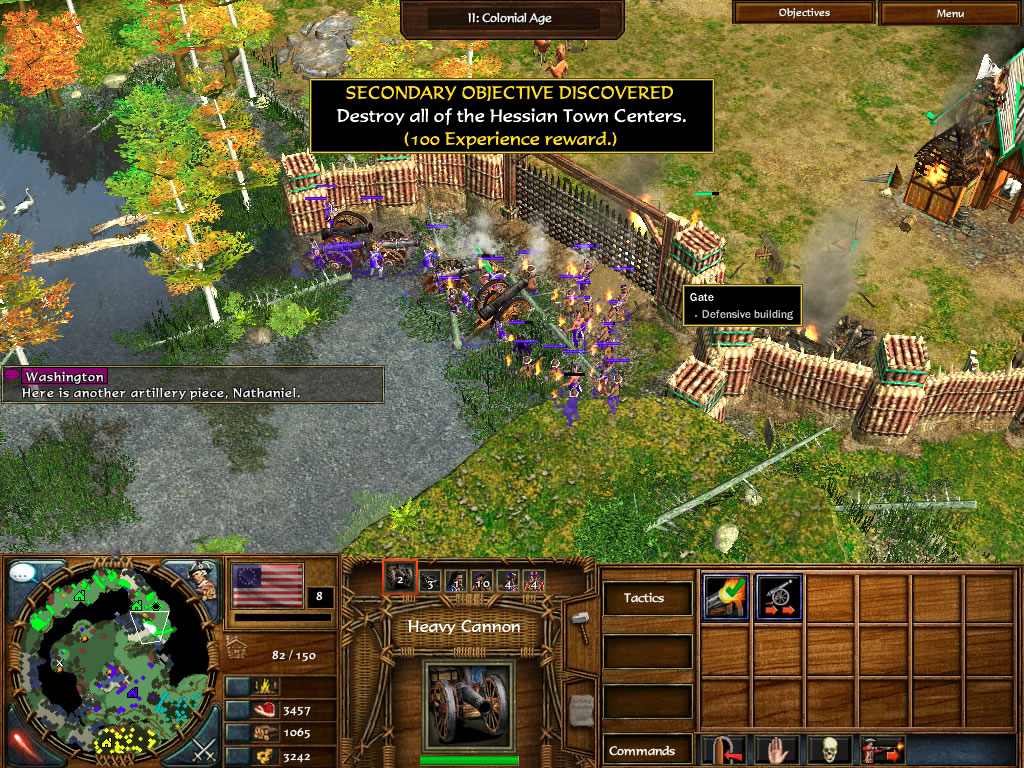
\includegraphics[width=5in]{images/age_of_empires_3.jpg}
\caption{Microsofts's \emph{Age of Empires III}: A real-time strategy interface \label{fig:aoe3}}
\end{center}
\end{figure}


The task list appears in the bottom right of the interface and displays icons for all available tasks, based on the currently-selected units. Some tasks, such as movement, require more information, which is provided by clicking on the main display with the mouse.

Information about the currently-selected units is displayed to the left of the task list. In the figure, a single heavy cannon unit has been selected, and information on its allegiance, player name, health, weaponry, and armor is shown.

A map of the entire game world, called the minimap, is displayed in the bottom left corner of the interface. This map shows the locations of all units, colored according to the controlling player, along with basic terrain type. Overlaid on the map is a representation of the field-of-view in the main display (white rectangle in Figure~\ref{fig:aoe3}). In Figure~\ref{fig:aoe3}, only the areas previously explored by the player are displayed in the minimap. % The world is of finite size in this game, and the minimap is fixed, both in size and viewpoint.

Clicking anywhere on the displayed part of the minimap moves the viewpoint in the main display to focus at that point. This option provides a quick way of moving the main display viewpoint around the (potentially large) virtual world. The minimap also displays primitive notifications; when a unit needs attention, a colored dot representing the unit flashes. A button, to the side of the minimap, centers the viewpoint of the main display on a unit currently without an assigned task, if one exists.

The interface in Figure~\ref{fig:aoe3} highlights notifications in two locations. Large notifications, in the center of the screen, provide urgent information to the user about the current objective. The larger notification is displayed on the screen for a short time before it is automatically hidden. Smaller notifications on the left side of the screen provide less urgent, actionable information to the user. The smaller notifications persist until dismissed by the user. When clicked the smaller notifications focus the camera on location in this case, a new piece of artillery.

Finally, a menu bar stretches across the top of the display. This displays current status in the top right (current quantities of resources), and it gives access to less-frequently-used functions, such as help screens and configuration dialogs.

% subsection real_time_strategy_games (end)
% section video_game_interfaces (end)


\section{Human-Robot Interaction}
\label{sec:hri}
Human-Robot Interaction (HRI) focuses on the interface between humans and robots. In their survey paper on HRI, Goodrich and Schultz introduce five attributes, shown in Figure~\ref{fig:five-attributes}, that define the interactions between humans and robots \cite{Goodrich_Survey}.

\begin{figure}[ht]
	\makebox[\textwidth]{\hrulefill}
	\begin{list}{$\bullet$}
		\item Level of behavior and autonomy
		\item \item Nature of information exchange % TODO: Why are two \item's needed?
		\item Structure of the team
		\item Adaptation, learning, and training of people and the robot
		\item Shape of the task
	\end{list}
	\makebox[\textwidth]{\hrulefill}
	\caption{Five attributes of Human-Robot Interaction \label{fig:five-attributes}}
\end{figure}

Of the five attributes of HRI, we will focus on autonomy and information exchange. Autonomy is defined as the extent of actions a robot may take independently. ``Sliding autonomy,'' the idea that autonomy may vary depending on context, is introduced in further detail in Section~\ref{sub:autonomy}. Information exchange describes the data that flows between a robot and a human. Like sliding autonomy, we introduce the idea that information exchange may vary based on context. Section~\ref{sub:info_exchange} introduces our refinements to the existing work in this field  \cite{Goodrich_Survey}.

\subsection{Autonomy}
\label{sub:autonomy}

The relationship between a robot and a human, as provided through the interface, can be viewed or conceptualized along the lines of a continuum or a scale of autonomy. Teleoperation represents one end of the spectrum, where the robot exhibits no qualities of autonomous behavior. On the other hand, a fully autonomous robot, acting independent of human input, represents the other extreme of autonomy. A simple scale of autonomy can be found in Figure~\ref{fig:autonomy} \cite{Goodrich_Survey}.

\begin{figure}[ht]
\begin{center}
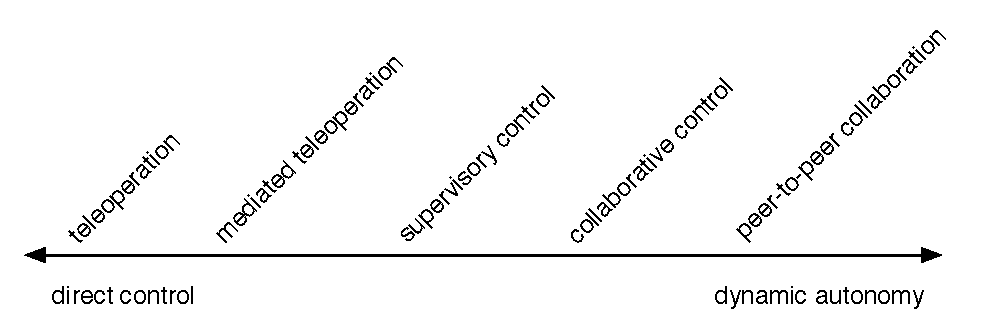
\includegraphics[width=5in]{images/autonomy.pdf}
\caption{Scale of Robot Autonomy\label{fig:autonomy}}
\end{center}
\end{figure}

Robots, as they presently exist, have a fairly limited set of autonomous actions available. As a result, most current interfaces are artificially conservative in their autonomy due to limitations in artificial intelligence. As research into artificial intelligence and machine learning grows, a much more diverse set of autonomous behaviors will inevitably become available. As user interface designers, we are tasked to create extensible interfaces to support future behaviors.

The idea of sliding autonomy allows a human, and a robot, to change the level of autonomy as needed. For illustration purposes, consider a robot that explores a warehouse. If the robot planned a poor navigation path, a user could manually specify the waypoints of an optimal path. If the robot is unable to complete the specified path due to an obstruction in the path, the robot could ask the user to directly teleoperate around the obstacle. Once free of the obstruction, the user would input a new set of goal coordinates and allow the autonomous navigation system to resume control. When combined with machine learning, sliding autonomy provides the robot an excellent platform for interactive learning from demonstration. The idea of interactive learning from demonstration is already well established \cite{GWAP} \cite{Grollman}.

\subsection{Information Exchange}
\label{sub:info_exchange}
The nature of information exchange defines the flow of data between the human and the robot. What information is provided, how it is represented, and when it is communicated are all properties of the interface design. This encompasses low-level communication of navigation and sensor data as well as high-level commands sent from the human \cite{Goodrich_Survey}. 

The purpose of visualization interfaces is to represent the one-way exchange of information from the robot to humans. This data typically includes location information, laser or sonar readings, battery readings, accelerometer readings, and map data. Original interfaces were written to be accessible programatically. These interfaces were slowly adapted to display sensor data graphically, but the resulting interfaces were disjointed and required operator training. Examples of these 2D user interfaces can be seen in Figure~\ref{fig:prior-hri} \cite{Bruemmer}.

\begin{figure}[ht]
\begin{center}
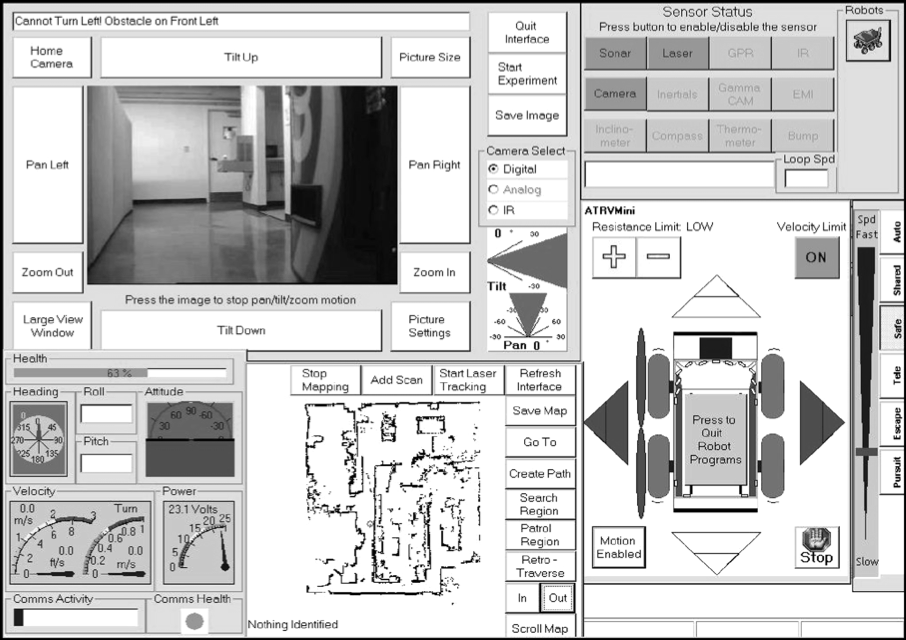
\includegraphics[width=5in]{images/prior-hri.png}
\caption{Existing Human-Robot Interface by Bruemmer et al
\label{fig:prior-hri}}
\end{center}
\end{figure}

In 2007, Nielsen introduced an ecological user interface with the goal of combining sensor data into a single, integrated display. Nielsen designed his interface for effective teleoperation, the technique of controlling a robot remotely. In his study, Nielsen compared an integrated 3D user interface to a simple 2D user interface for several environment-searching tasks. The 3D user interface displayed combined sensor data through a single viewport, while the 2D user interface displayed the same data through individual elements. The study found the 3D interface decreased collisions and decreased task completion time \cite{Nielsen_Teleoperation}.

Nielsen attributes the success of the 3D interface to improved situational awareness. The observed effect of situational awareness and context on interface effectiveness is congruous with the findings of other researchers \cite{Nielsen_Teleoperation}.

A limitation of Nielsen's interface is that its focus on teleoperation leaves the robot without autonomy. While teleoperation may be optimal for single robot environments it does not allow for concurrent robot control. This limitation requires a human operator for every active robot. We believe that providing an ecological interface common to multiple robots allows for more efficient use of human resources.

% chapter hci (end)
